%!TEX root = ../terrainbook.tex

\graphicspath{{acquisition/}}

\chapter{Acquisition of elevation measurements}
\label{chap:acquisition}

The very first step in the process of terrain modelling is the acquisition of elevation measurements. 
Nowadays, these measurements are usually collected in large quantities using some form of remote sensing, \ie\ sensors that measure---in our case---the distance to the Earth's surface from an airborne or even a spaceborne platform. 
In raw form elevation measurements are typically stored as a point cloud, \ie\ a collection of georeferenced 3D points with each point representing one elevation measurement on the Earth's surface.

As with any kind of real-world measurement, there are various uncertainties and restrictions that lead to distortions---called \emph{artefacts}---in the acquired data. 
This often makes further processing of the data more difficult, because these artefacts often violate assumption that are made in the DTM algorithms used to further process and analyse the point cloud, leading to erroneous results. 
It is important that you are aware of these artefacts while working with elevation data, because only then you will be able to make the right modelling decisions. 
%Section~\ref{sec:artefacts} gives an overview of common problems in elevation data.


\section{Acquisition techniques}
\label{sec:acquisistion-techniques}
There are a number of remote sensing techniques that are used to measure elevation on Earth or other planets. 
Typically, these techniques measure 1) the distance to the target surface and 2) their own position and orientation with respect to some global reference system. 
By combining these, we can compute the 3D coordinates of the measured location on the target surface. 

The position and orientation of the sensor is usually measured respectively using a global navigation satellite system (GNSS) such as GPS and an inertial measurement unit (IMU).
Only in case of spaceborne sensors GNSS is not available, and instead a star tracker is used.

How distance is measured depends on the sensor technique. 
What follows is a brief description of the four main techniques used in practice. 

\begin{figure}
	\centering
	\begin{subfigure}{0.4\linewidth}
		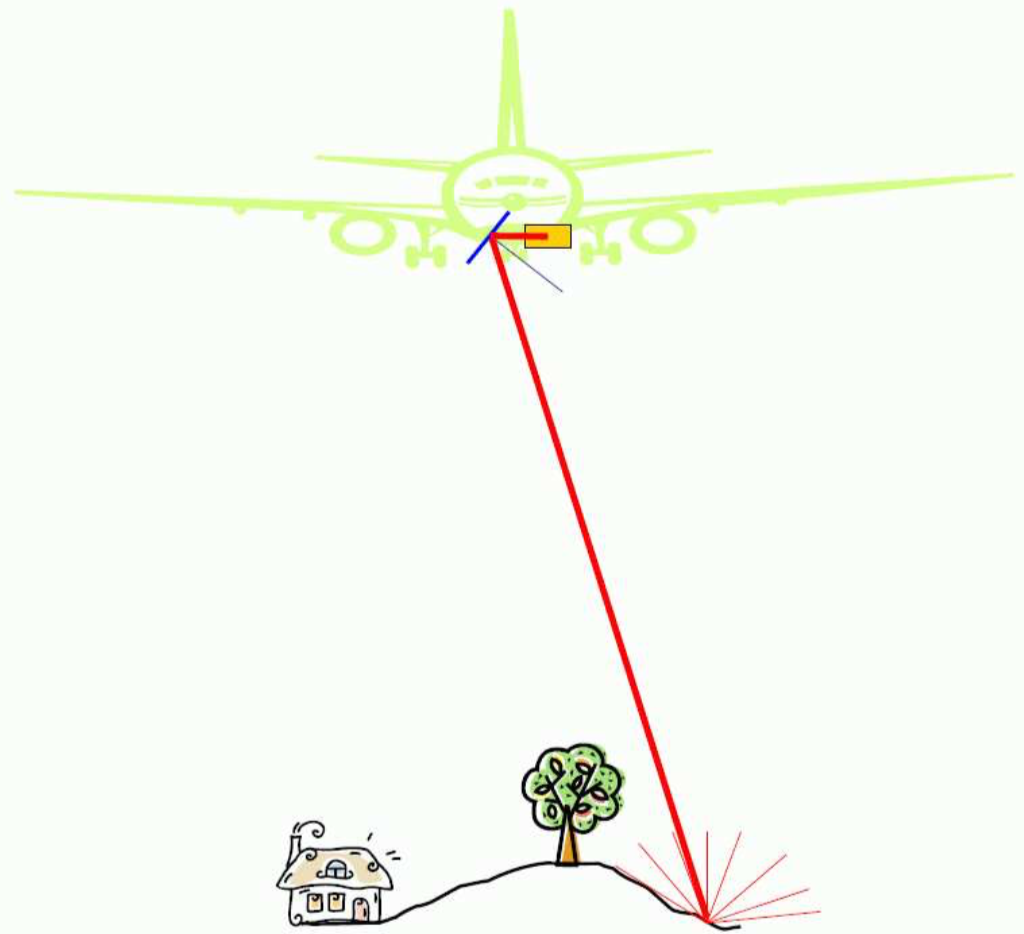
\includegraphics[width=\textwidth]{figs/lidar.png}
		\subcaption{Lidar}
		\label{fig:acqLidar}
	\end{subfigure}
	\quad
	\begin{subfigure}{0.4\linewidth}
		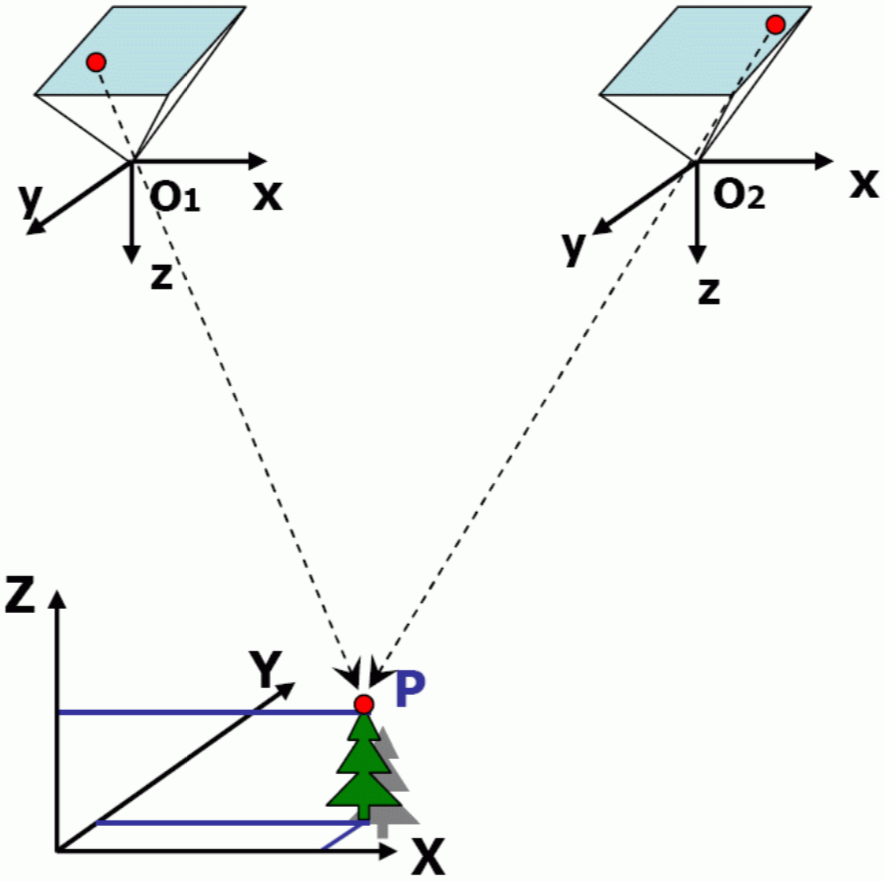
\includegraphics[width=\textwidth]{figs/photogrammetry.png}
		\subcaption{Photogrammetry}
		\label{fig:acqPhoto}
	\end{subfigure}
	\caption{Two sensors techniques for DTM acquisition}
	\label{fig:sensors}
\end{figure}
% FIXME image with flight parameters and strips

\subsection{Lidar}
A lidar system\footnote{While `lidar' is often treated as the acronym of \textbf{li}ght \textbf{d}etection \textbf{a}nd \textbf{r}anging, it actually originated as a portmanteau of `light' and `radar'. Source \url{https://en.wikipedia.org/wiki/Lidar\#History\_and\_etymology}} measures distance to a target by illuminating it with pulsed laser light and measuring the reflected pulses with a sensor (see Figure~\ref{fig:acqLidar}). 
It is generally considered to be the most accurate acquisition technique.
By measuring the time-of-flight, \ie\ the difference in time between sending a pulse and sensing its return, the distance to the target that reflected the pulse can be found by multiplying the time-of-flight with the speed of light, which is a known constant.
Lidar thus makes use of the natural phenomenon of \emph{backscattering}, \ie\ the reflection of (electromagnetic) waves or signals back to the direction they came from. 
%The strength of the return signal, \ie~its intensity, is also recorded for each point.
%Most often an infra-red laser is used, but sometimes another wavelengths is used. 
When equipped with a green laser, lidar is also suitable for bathymetry because that wavelength has the special ability to penetrate water and detect the sea floor. For above water terrain usually a near-infrared laser is employed.

For a given laser pulse, a lidar system can record multiple returns. 
For instance, when a pulse hits a leaf on a tree, part of the signal is immediately reflected (the first return) while another part of the signal penetrates the leaf and travels further until it hits the ground and reflects back to the sensor (the second and in this case last return).  
This gives lidar the unique ability to sense a ground surface from the air, even when it is covered with a forest, making it particularly suitable for highly vegetated areas.

On Earth, for DTM generation, only airborne lidar is used, attached to either planes or helicopters.
However for celestial bodies that do not have an atmosphere (such as the Moon), lidar can also be used from space\footnote{NASA has used lidar on the Moon (\url{https://lola.gsfc.nasa.gov}) and on Mars (\url{https://en.wikipedia.org/wiki/Mars_Orbiter_Laser_Altimeter}).}.

\begin{link-box}
This YouTube video explains the principles of an aerial LiDAR system:
\\
\url{https://youtu.be/EYbhNSUnIdU}
\end{link-box}


% TODO : put a side-by-side with vegetation and without lidar to show DTM and DSM


\subsection{Photogrammetry}
Photogrammetry allows us to measure the distance from overlapping photographs taken from different positions. 
If a ground point, called a \emph{feature}, is identifiable in two or more images, its 3D coordinates can be computed in two steps. 
First, a viewing ray for that feature must be reconstructed for each image. 
Photogrammetry allows us to measure distance from overlapping photographs taken from different positions. 
First, a viewing ray for that feature must be reconstructed for each image. 
A viewing ray can be defined as the line from the feature, passing through the projective centre of the camera, to the corresponding pixel in the image sensor (see Figure~\ref{fig:acqPhoto}). 
Second, considering that we know the orientation and position of the camera, the distance to the feature (and its coordinates) can be computed by calculating the spatial intersection of several viewing rays.

% interior orientation (camera parameters such as focal length) and the exterior orientation (camera position and orientation)

The number of 3D point measurements resulting from photogrammetry thus depends on the number of features that are visible in multiple images, \ie\ the so-called \emph{matches}.
With \emph{dense image matching} it is attempted to find a match for every pixel in an image. 
If the \emph{ground sampling distance}, \ie\ the pixel size on ground level, is small (around 5cm for state-of-the-art systems), point densities of hundreds of points per square meter can be achieved, which is much higher than the typical lidar point cloud (typically up to dozens of points per square meter). 

In photogrammetry we distinguish between \emph{nadir} images, that are taken in a direction straight down from the camera, and \emph{oblique} images that are taken at an angle with respect to the nadir direction.
Vertical features such as building facades are only visible on oblique images.
Therefore, oblique images are needed if one wants to see building facades in a dense image matching point cloud.

Because photography is used, photogrammetry gives us also the colour of the target surface, in addition to the elevation.
This could be considered an advantage over lidar which capture several attributes for each point (\eg\ the intensity of measured laser pulse and the exact GPS time of measurement), but colour is not among them.

Both airborne and spaceborne photogrammetry are possible.

\subsection{InSAR}
Interferometric synthetic aperture radar (InSAR) is a radar-based technique that is used from space in the context of DTM generation. 
It is quite different from airborne lidar or photo\-gramme\-try-based DTM acquisition because of the extremely high altitude of the satellite carrying the sensor. 
Signals have to travel very long distances through several layers of unpredictable atmospheric conditions. 
As a result the speed of the radar signal is not known and the time-of-flight principle can not be used. 
However, by using a comprehensive chain of processing operations based on the measured phase shifts and the combination of multiple InSAR images, elevation can still be measured. 
With InSAR it is possible to cover very large regions in a short amount of time, \eg\ the global SRTM\footnote{\url{https://en.wikipedia.org/wiki/Shuttle_Radar_Topography_Mission}} dataset was generated with InSAR\@. 
Compared to dense image matching and lidar, InSAR-derived DTMs usually have a much lower resolution, \eg\ SRTM has a pixel size of 30 meters.

\begin{link-box}
The principles of InSAR\@.

\url{https://en.wikipedia.org/wiki/Interferometric_synthetic-aperture_radar}
\end{link-box}

\subsection{Echo sounding}
\label{sec:mbes}
Echo sounding is a form of sonar that can be used for bathymetry, \ie\ mapping underwater terrains from a boat. 
Similar to lidar, it uses the time-of-flight principle to compute distance, but sound is used instead of light. 

Single-beam and multi beam echo sounders exist. Multi-beam systems are capable of receiving many narrow sound beams from one emitted pulse. As a result it measures the target surface much more accurately. 
For bathymetry usually a multi-beam echo sounder is used.

\begin{link-box}
  The principles of echo sounding.
  \\
  \url{https://en.wikipedia.org/wiki/Echo_sounding}
\end{link-box}




\section{Artefacts}
\label{sec:artefacts}
There are many aspects, both in our control as not in our control, in the acquisition process that affect the quality and usability of the resulting elevation data for a given application. Some examples are
\begin{itemize}
	\item the choice of sensor technique, 
	\item the sensor specifications, \eg\ the resolution and focal length of a camera, or the scanning speed, the width of the swath, and scanning pattern of a lidar system,
	\item the flight parameters, \eg\ the flying altitude and the distance and overlap between adjacent flights,
	\item atmospheric conditions, 
	\item the physical properties of the target surface.
\end{itemize}

An artefact is any error in the perception or representation of information that is introduced by the involved equipment or techniques. 
Artefacts can result in areas without any measurements (\eg\ the \emph{no-data} values in a raster), or in so-called \emph{outliers}, \ie\ sample points with large errors in their coordinates. 

We distinguish three types of artefacts, 1) those that occur due to problems in the sensor, 2) those that occur due to the geometry and material properties of the target surface, and 3) those that occur due to post-processing steps.

% Active/passive sensors
% different platforms ground/airborne/space
% different physical principles
% pulse footprint, wavelength
% different sensor specs (resolution, speed) and operation specs (flight height etc)
% different cost, update cycles

\subsection{Sensor}
The sensor position and orientation is continuously monitored during acquisition, \eg\  by means of GNSS and an IMU for airborne and seaborne systems, and used to determine the 3D coordinates of the measured points. 
Consequently, any errors in the position and orientation of the sensor platform affect the elevation measurements. 
For this reason adjacent flight strips (see Figure~\ref{fig:lidarStrips}) often need to be adjusted to match with each other using ground control points. 
\begin{figure}
	\centering
	\begin{subfigure}{0.4\linewidth}
		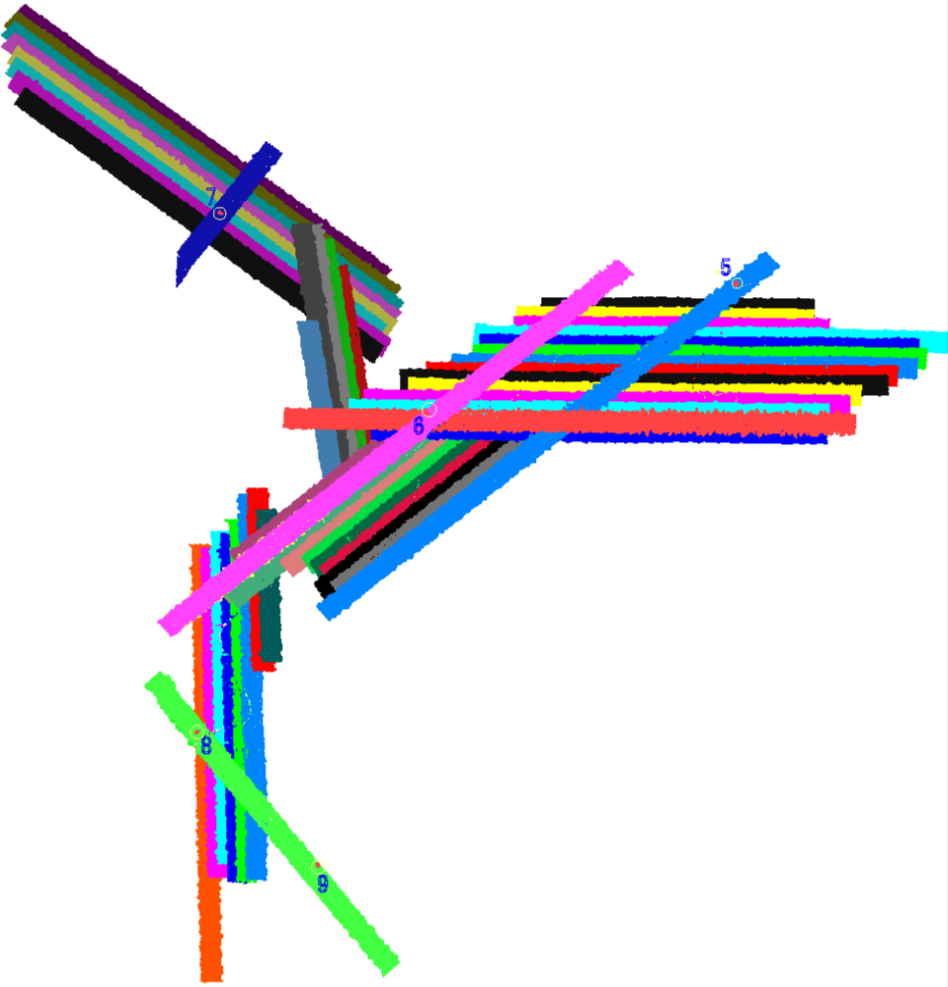
\includegraphics[width=\textwidth]{figs/lidar_strips.png}
		\subcaption{Plan view of the different strips of a lidar survey \citep{Kornus03}}
		\label{fig:lidarStrips}
	\end{subfigure}
	\quad
	\begin{subfigure}{0.4\linewidth}
		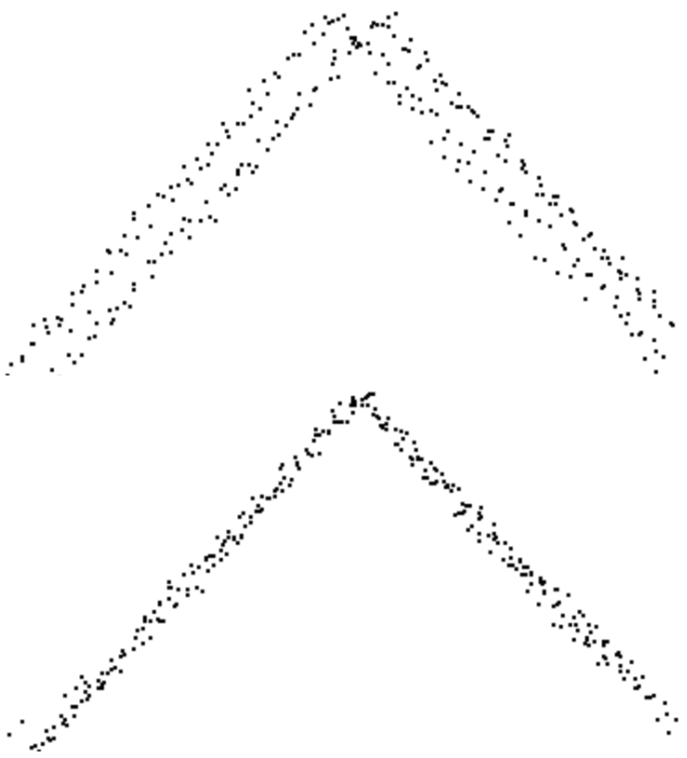
\includegraphics[width=\textwidth]{figs/strip_adjustment.png}
		\subcaption{Cross-section of gable roof before (top) and after (bottom) strip adjustment \citep{Vosselman02}}
		\label{fig:lidarGableRoof}
	\end{subfigure}
	\caption{Strip adjustment for lidar point clouds}
	\label{fig:lidarStripAdj}
\end{figure}
If the strip adjustments process fails or is omitted, a `ghosting' effect can occur as illustrated in Figure~\ref{fig:lidarGableRoof} (top). 
Photogrammetry knows a similar process called aerial triangulation, in which camera positions and orientation parameters (one set for each image) are adjusted to fit with each other. Errors in the aerial triangulation is can lead to a noisy result for the dense matching as seen in Figure~\ref{fig:dim}.
\begin{figure}
	\centering
	\begin{subfigure}{0.95\linewidth}
		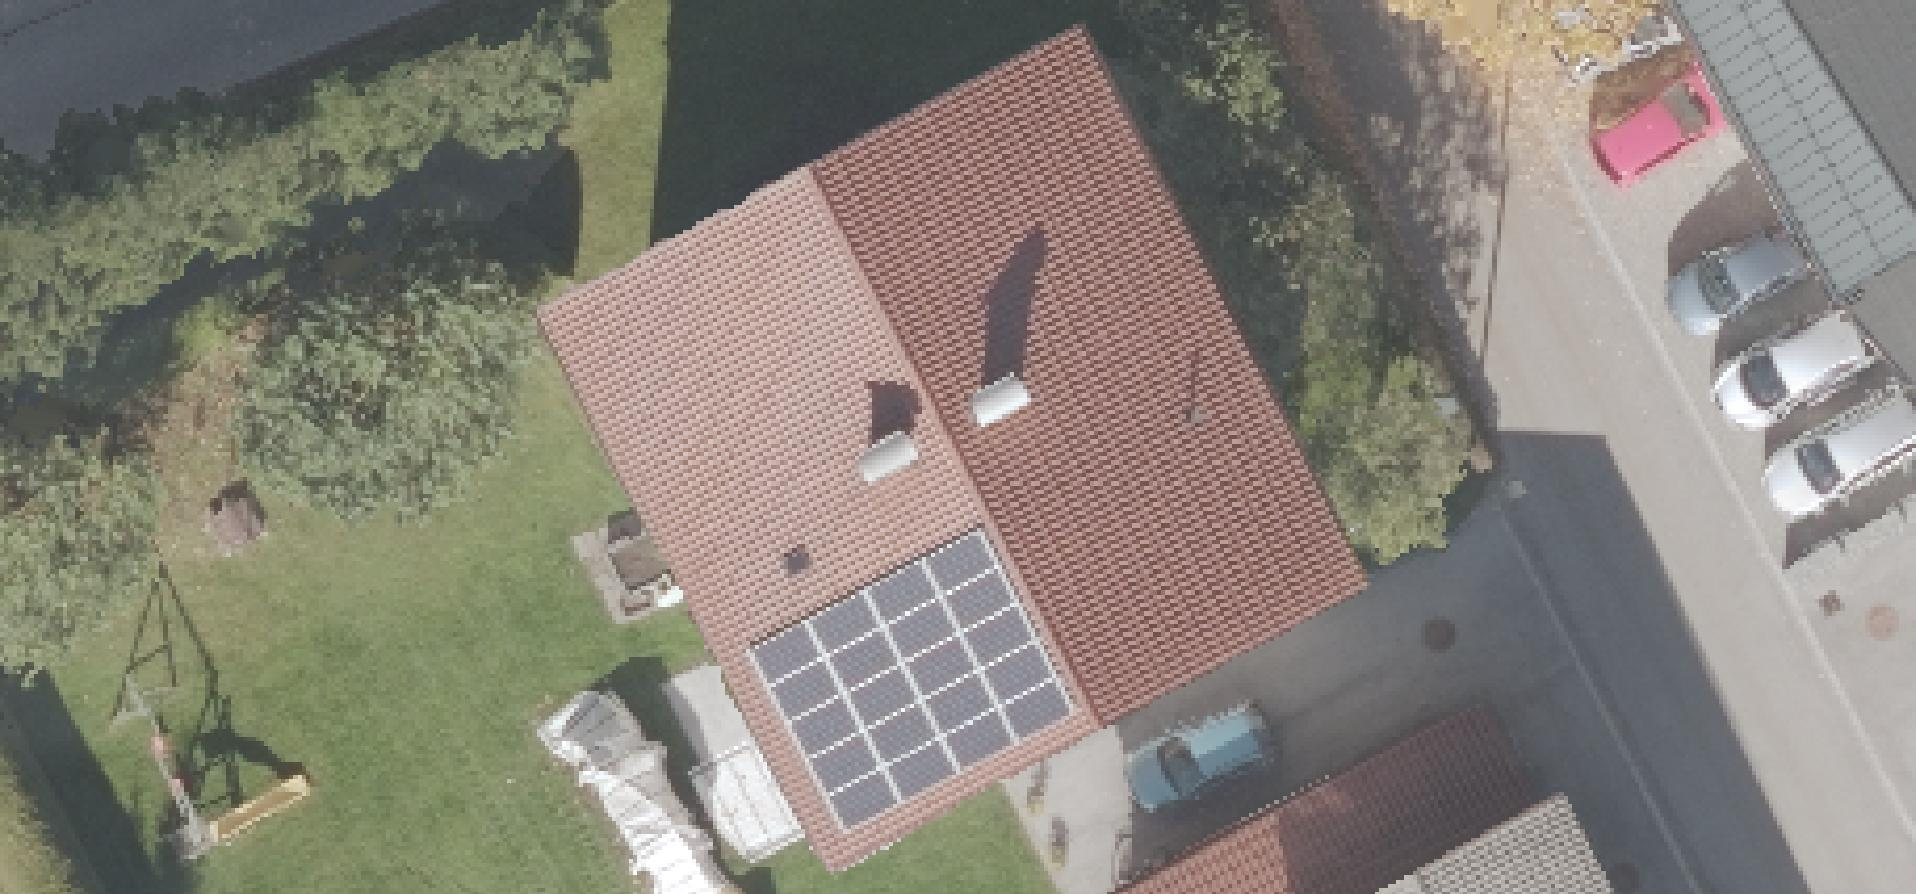
\includegraphics[width=\textwidth]{figs/Roof_OP_NA_10cm.jpg}
		\subcaption{Nadir image}
		\label{fig:dim:a}
	\end{subfigure}
	
	\begin{subfigure}{0.95\linewidth}
		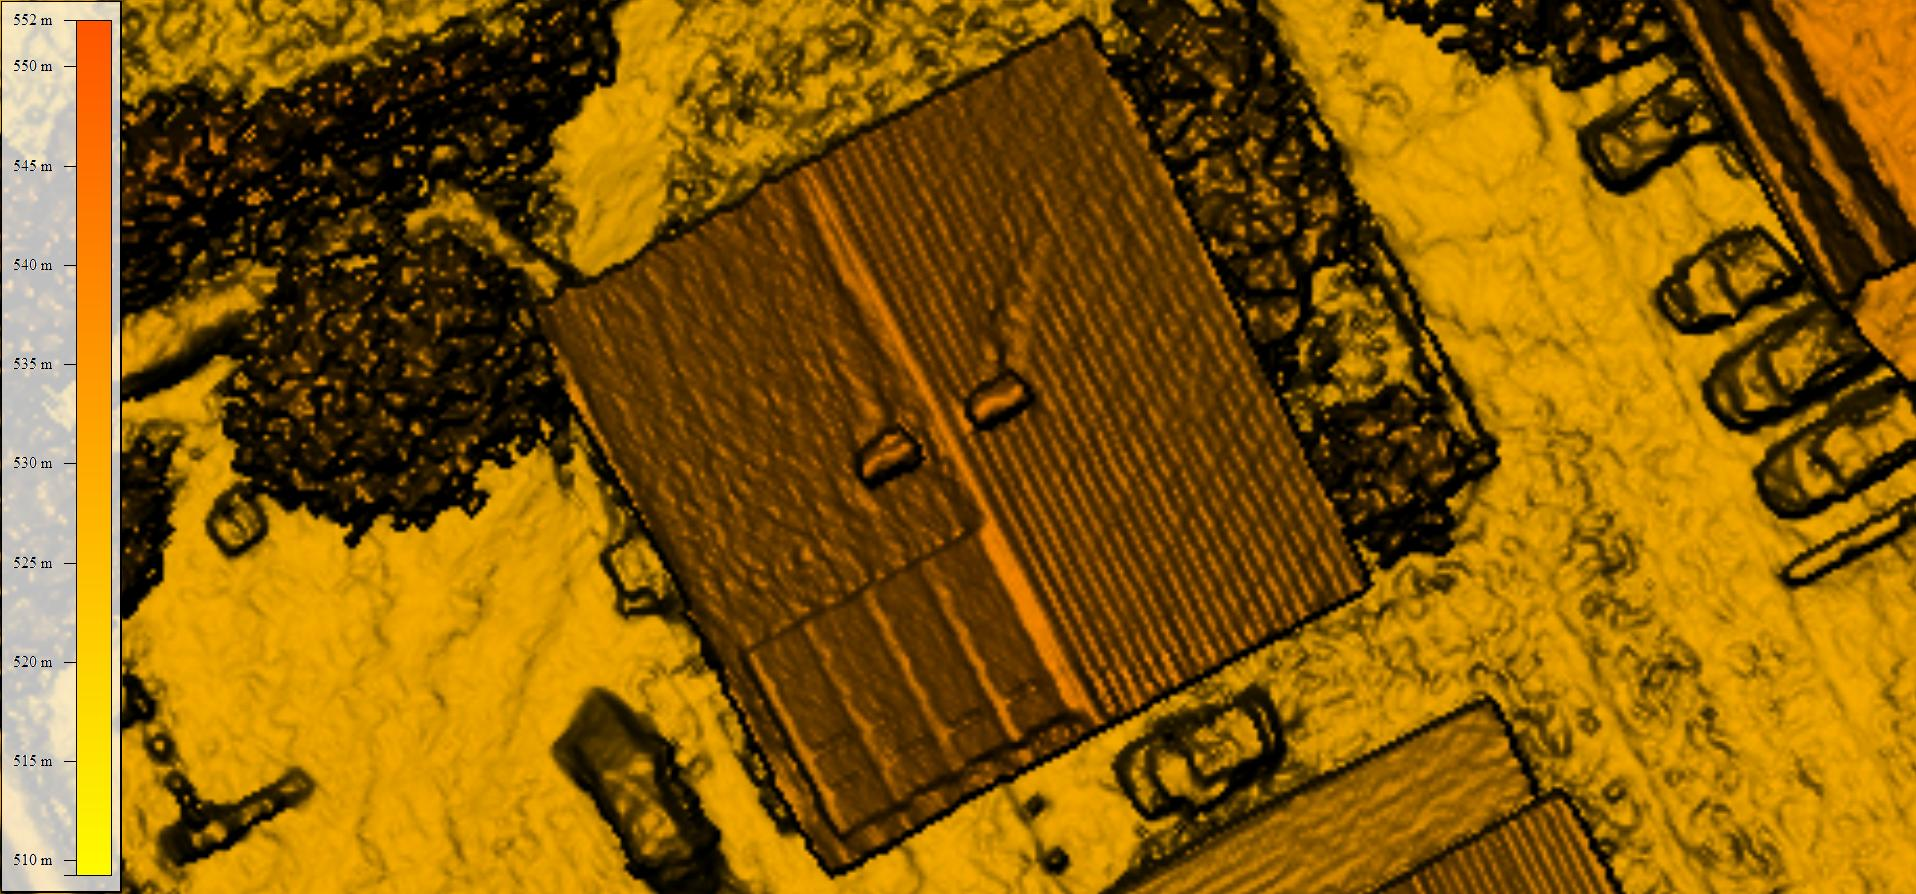
\includegraphics[width=\textwidth]{figs/Roof_DSM_NA_10cm.jpg}
		\subcaption{DSM with good aerial triangulation}
		\label{fig:dim:b}
	\end{subfigure}
	
	\begin{subfigure}{0.95\linewidth}
		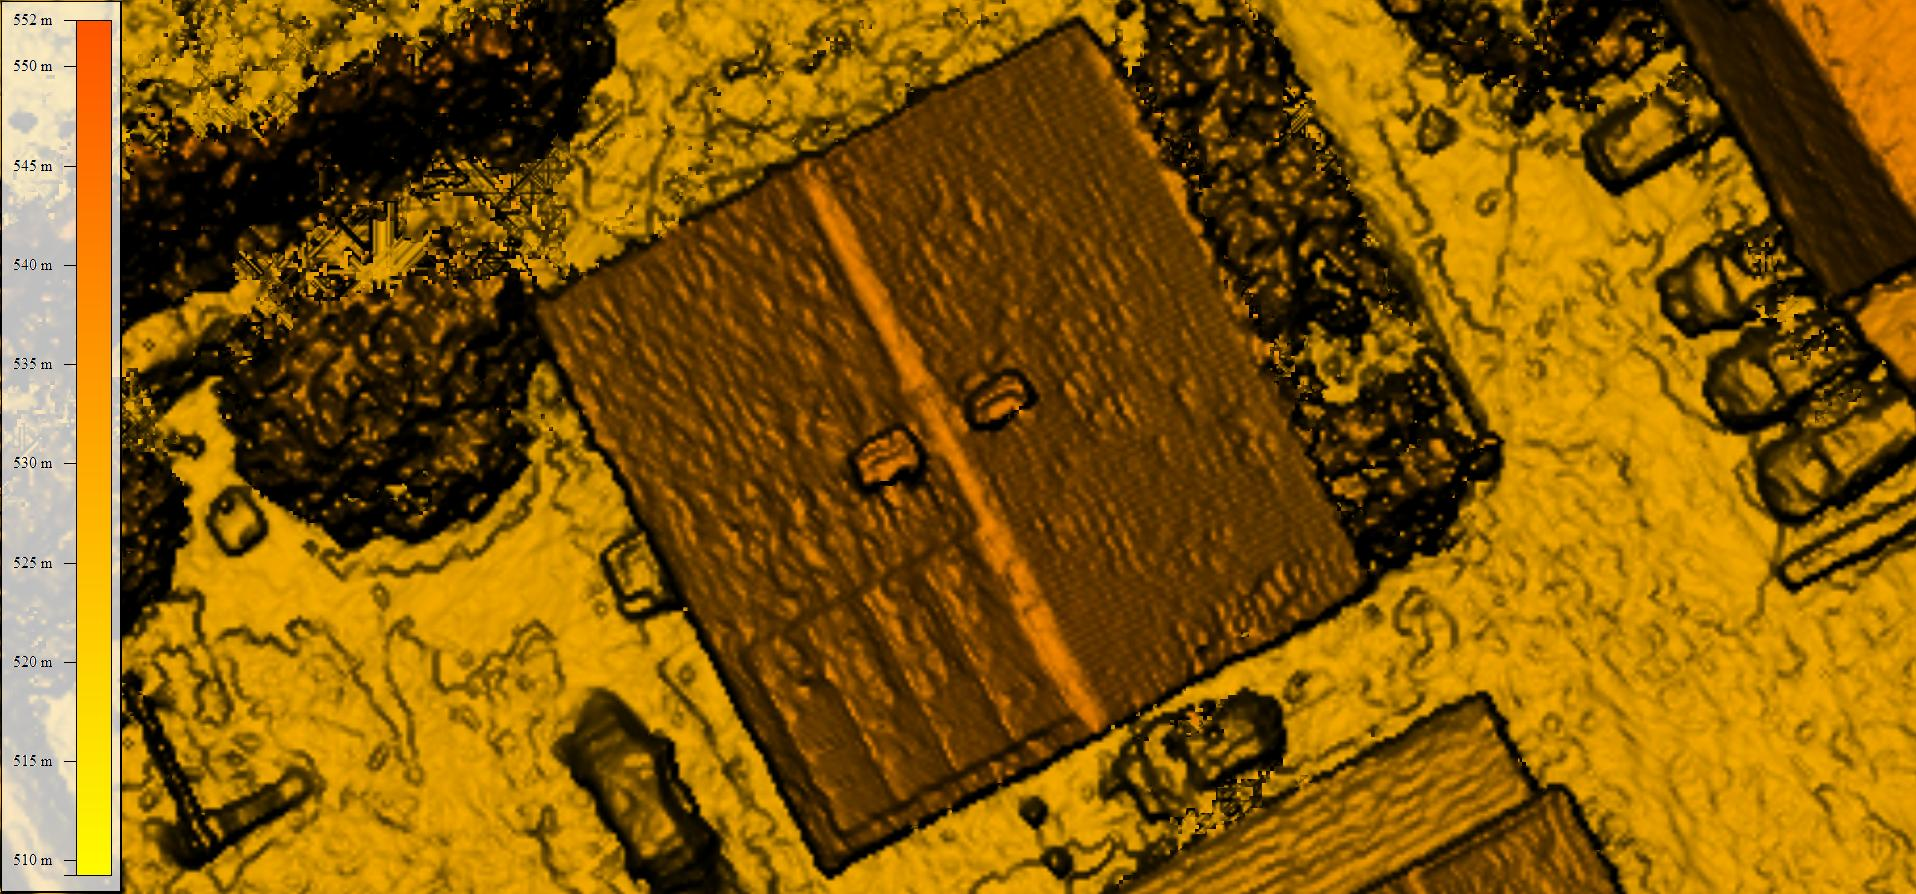
\includegraphics[width=\textwidth]{figs/Roof_DSM_NA+OBL_10cm.jpg}
		\subcaption{DSM with poor aerial triangulation}
		\label{fig:dim:c}
	\end{subfigure}
	\caption{Errors in aerial triangulation can lead to distortions in the DSM (derived from dense image matching). Images courtesy of Vermessung AVT.}
	\label{fig:dim}
\end{figure}


\subsection{Target surface}
Many commonly occurring  artefacts  happen due to properties of the target surface. We distinguish three classes.

\subsubsection{Geometry} 
The shape of the target surfaces in relation to the sensor position has a great effect on 1) local point densities and 2) occlusion. 
As you can see from Figure~\ref{fig:lidarAcquisitionConditions:a}, which illustrates this for lidar, surfaces that are closest to the scanner and orthogonal to the laser beams will yield the highest point densities (see the rooftop of the middle house). 
\begin{figure}
	\centering
	\begin{subfigure}{0.4\linewidth}
		\includegraphics[width=\textwidth,page=2]{figs/lidarAcq.pdf}
		\subcaption{Point distribution and occlusion}
		\label{fig:lidarAcquisitionConditions:a}
	\end{subfigure}
	\quad
	\begin{subfigure}{0.3\linewidth}
		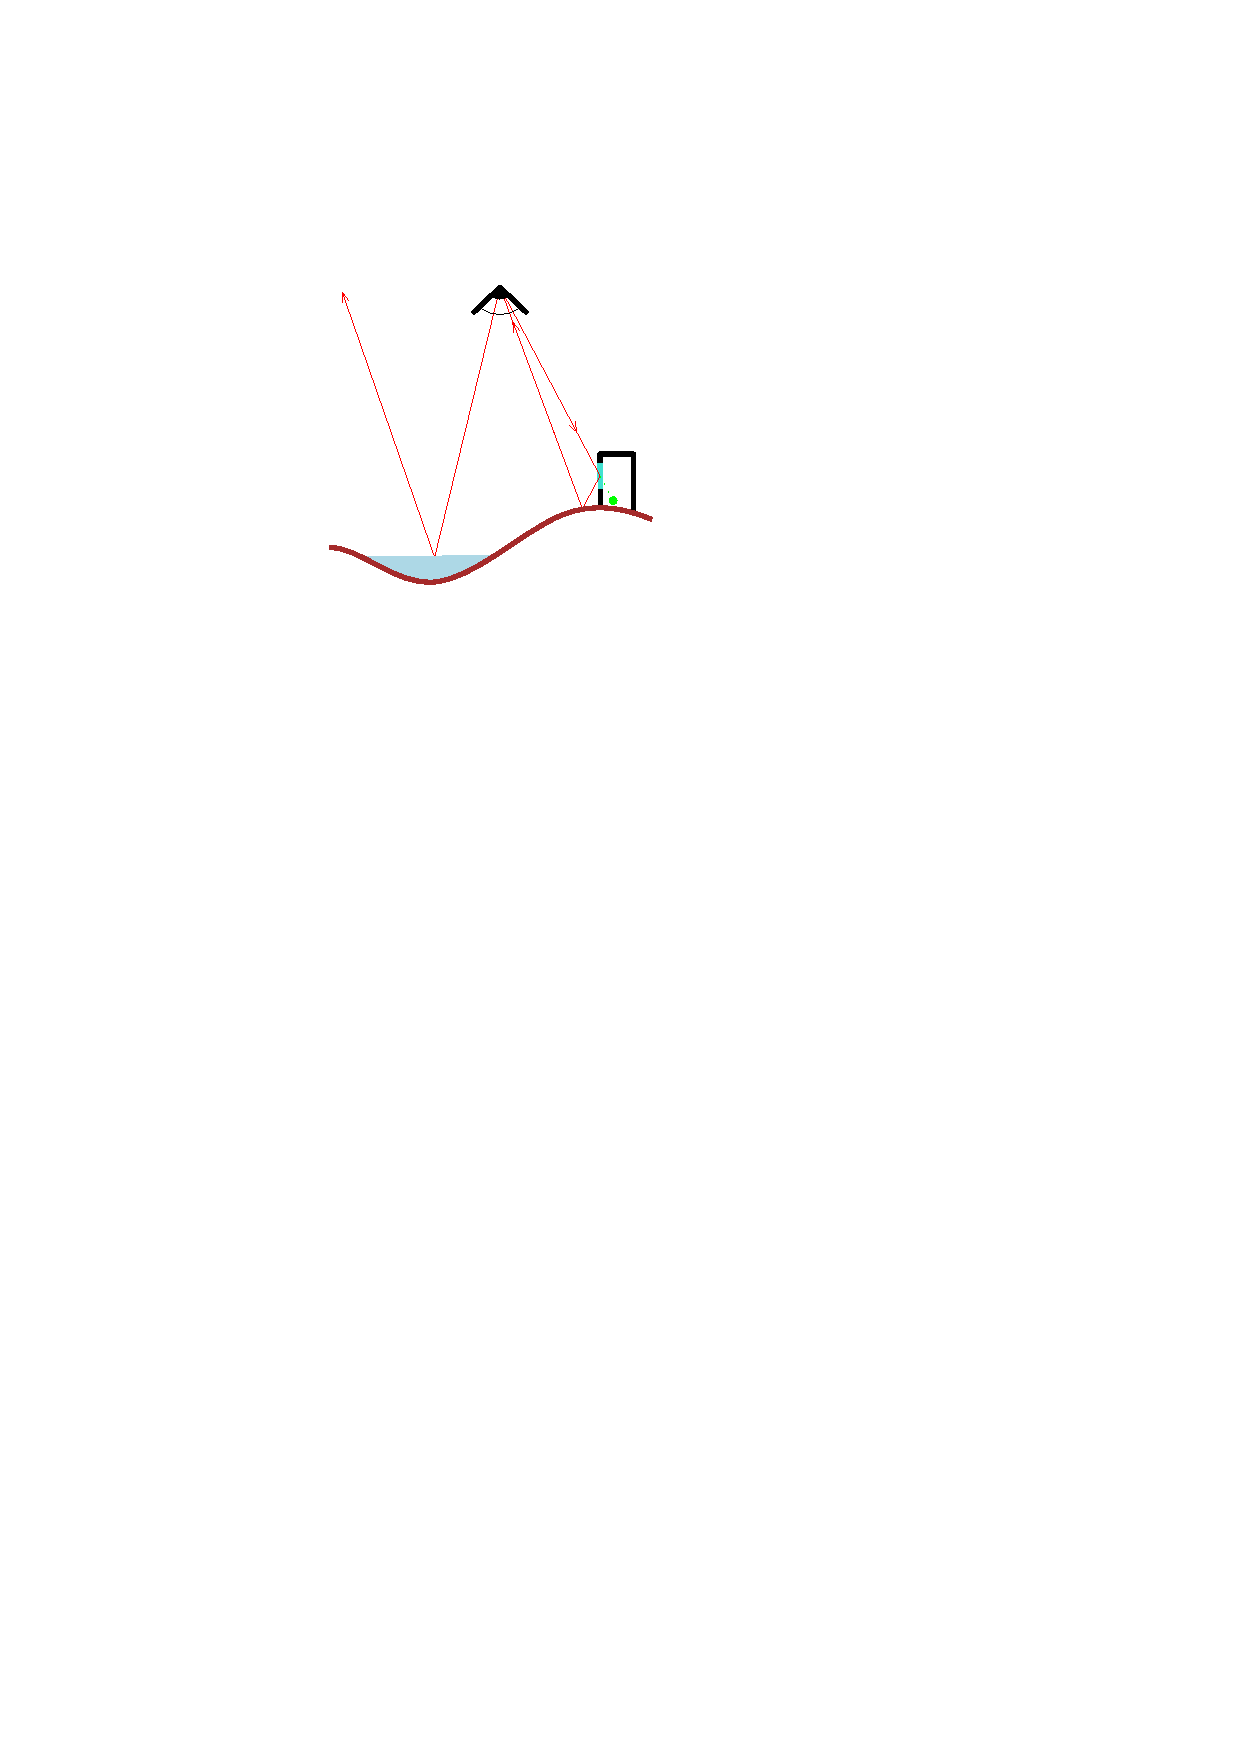
\includegraphics[width=\textwidth,page=1]{figs/lidarAcq.pdf}
		\subcaption{Reflection and multi-path}
		\label{fig:lidarAcquisitionConditions:b}
	\end{subfigure}
	\caption{Sources of artefacts in lidar point clouds}
	\label{fig:lidarAcquisitionConditions}
\end{figure}
Very steep surfaces on the other hand, yield relatively low point densities (see the façades of the buildings). 

Occlusion happens when a surface is not visible from the scanner position. 
As a result there will be gaps in the point coverage, also visible in Figure~\ref{fig:lidarAcquisitionConditions:a}. 
Notice how some steep surfaces and some of the adjacent ground are not registered at all by the scanner because it simply could not `see' these parts.

The severity of both effects mostly depends on the geometry of the target objects and flight parameters such as the flying altitude and the amount of overlap between flight strips.
However, regardless of what flight parameters are chosen for a survey both effects are almost always visible somewhere in the resulting dataset, see for example Figure~\ref{fig:pcd} for different lidar datasets for the same area.

% oblique vs nadir for occlusion
%Especially occlusion can be a problem for (2.5D) DTM generation because it causes no-data areas that may be problematic.

\begin{figure}
	\centering
	\begin{subfigure}{0.45\linewidth}
		
\includegraphics[width=\textwidth]{figs/ahn1_d.png}
		\subcaption{AHN1 (1996-2003)}
		\label{fig:pcd:ahn1}
	\end{subfigure}
	\quad
	\begin{subfigure}{0.45\linewidth}
		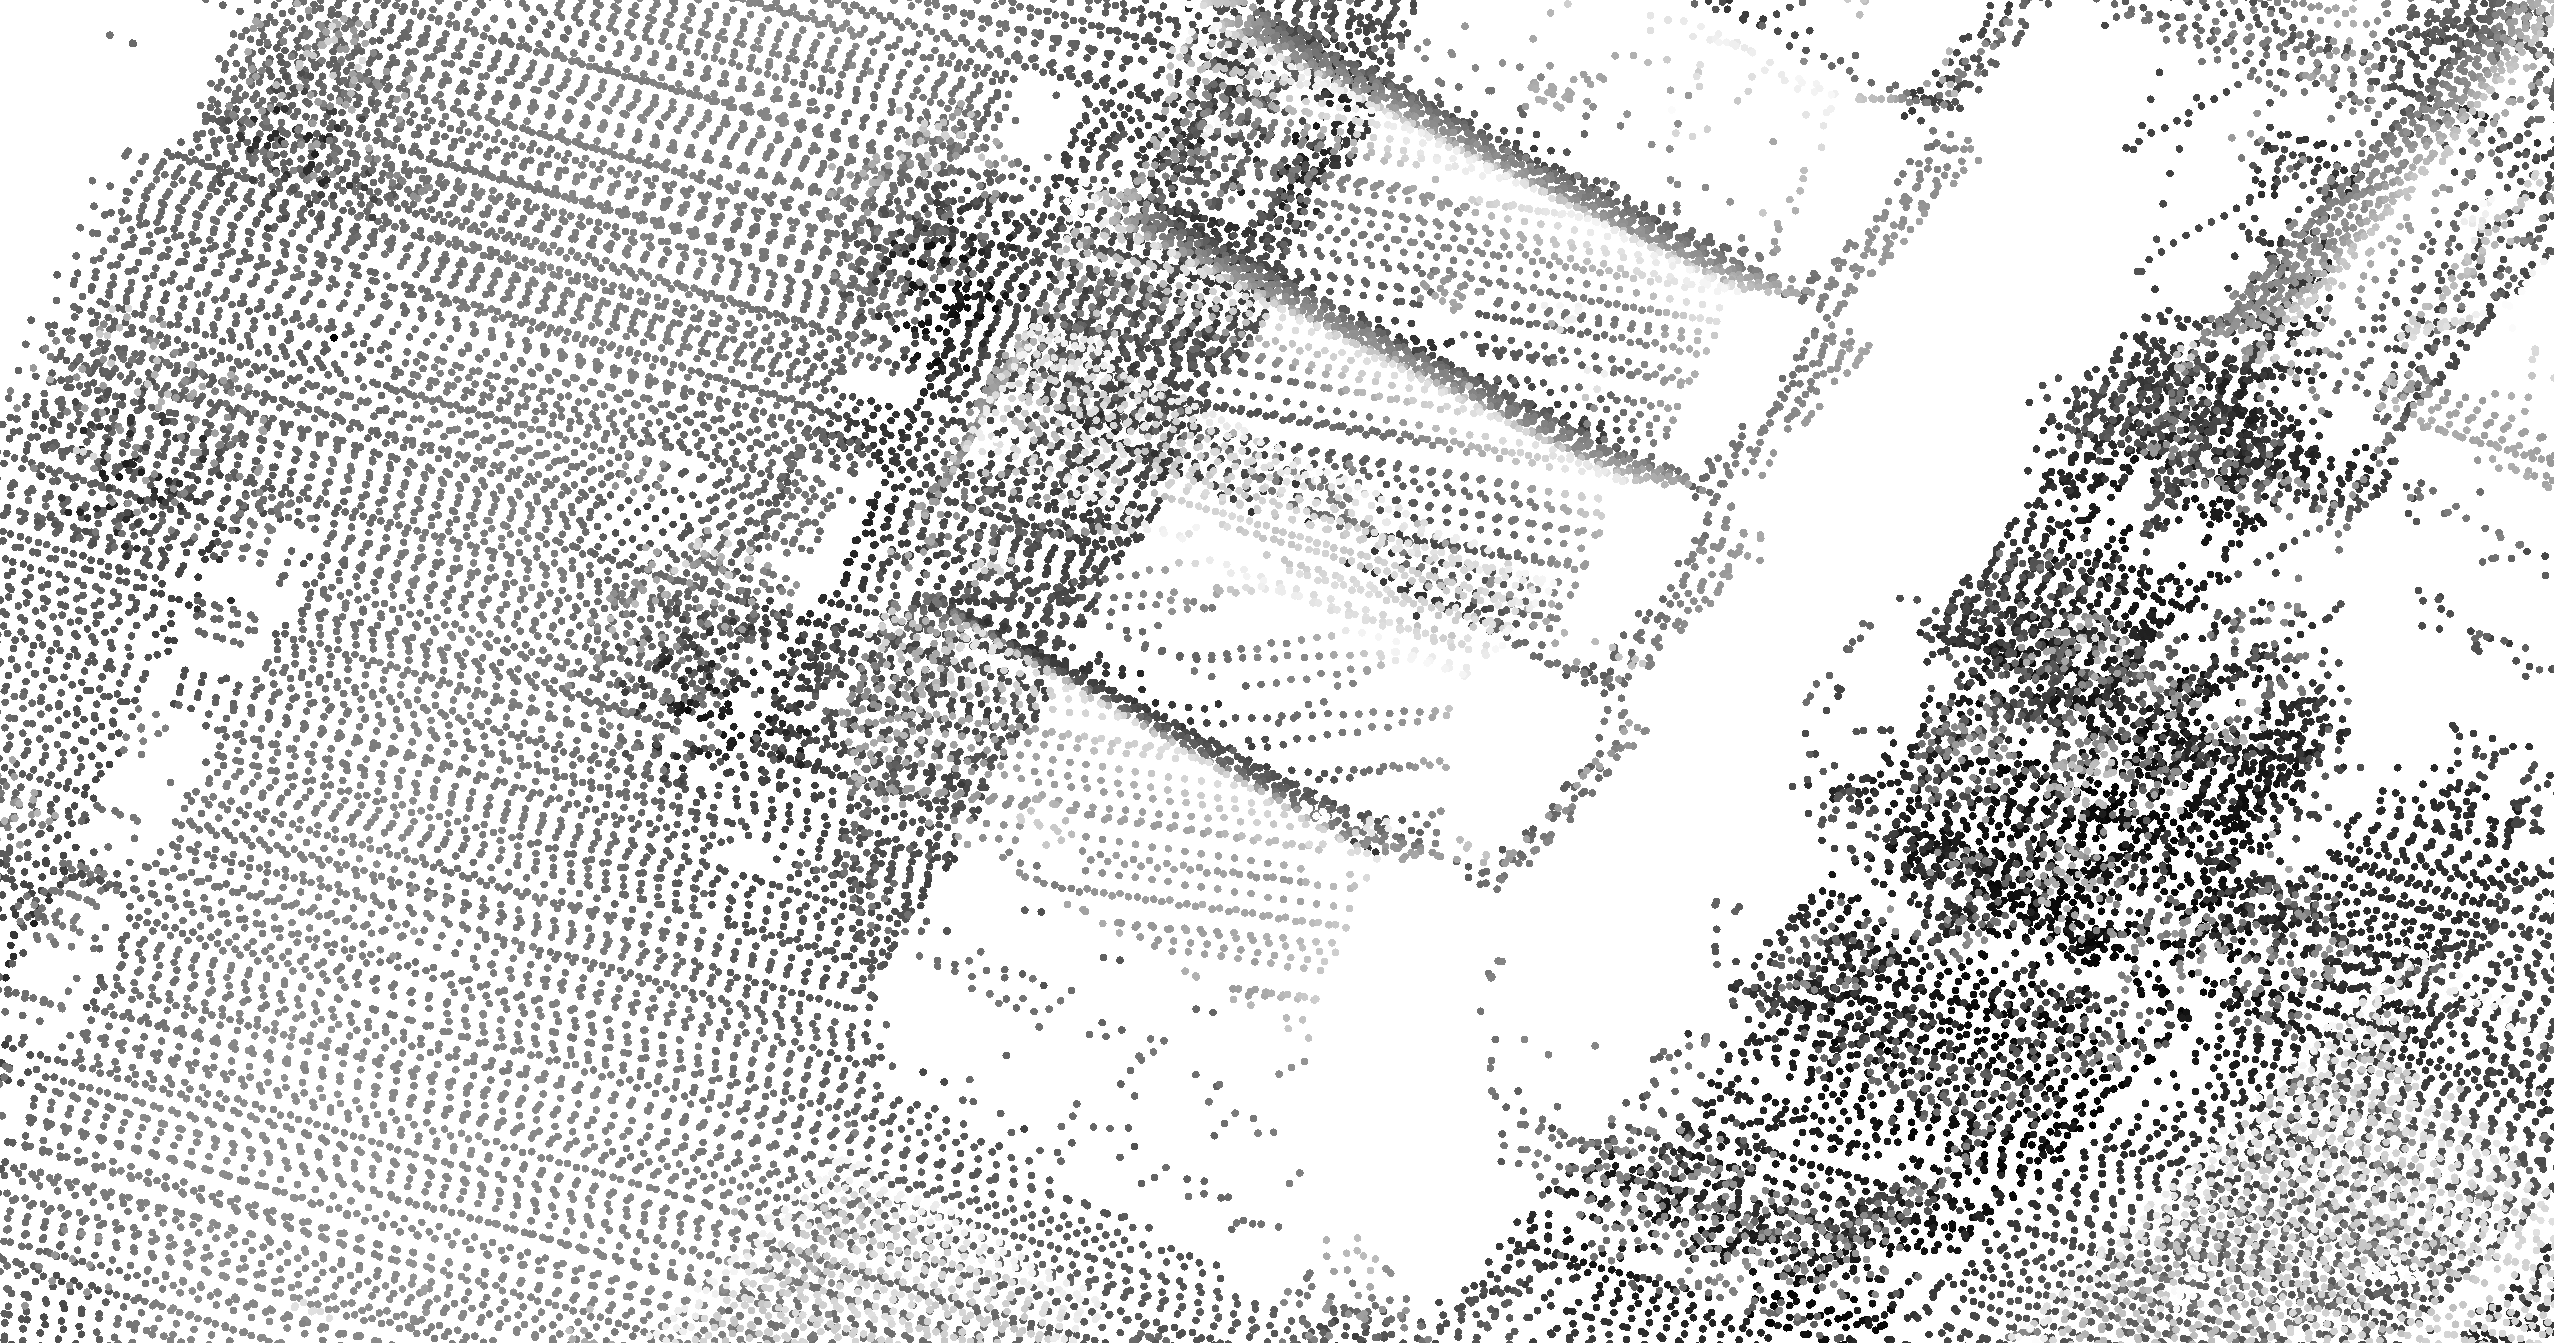
\includegraphics[width=\textwidth]{figs/ahn2_d.png}
		\subcaption{AHN2 (2008)}
		\label{fig:pcd:ahn2}
	\end{subfigure}
	
	\begin{subfigure}{0.45\linewidth}
		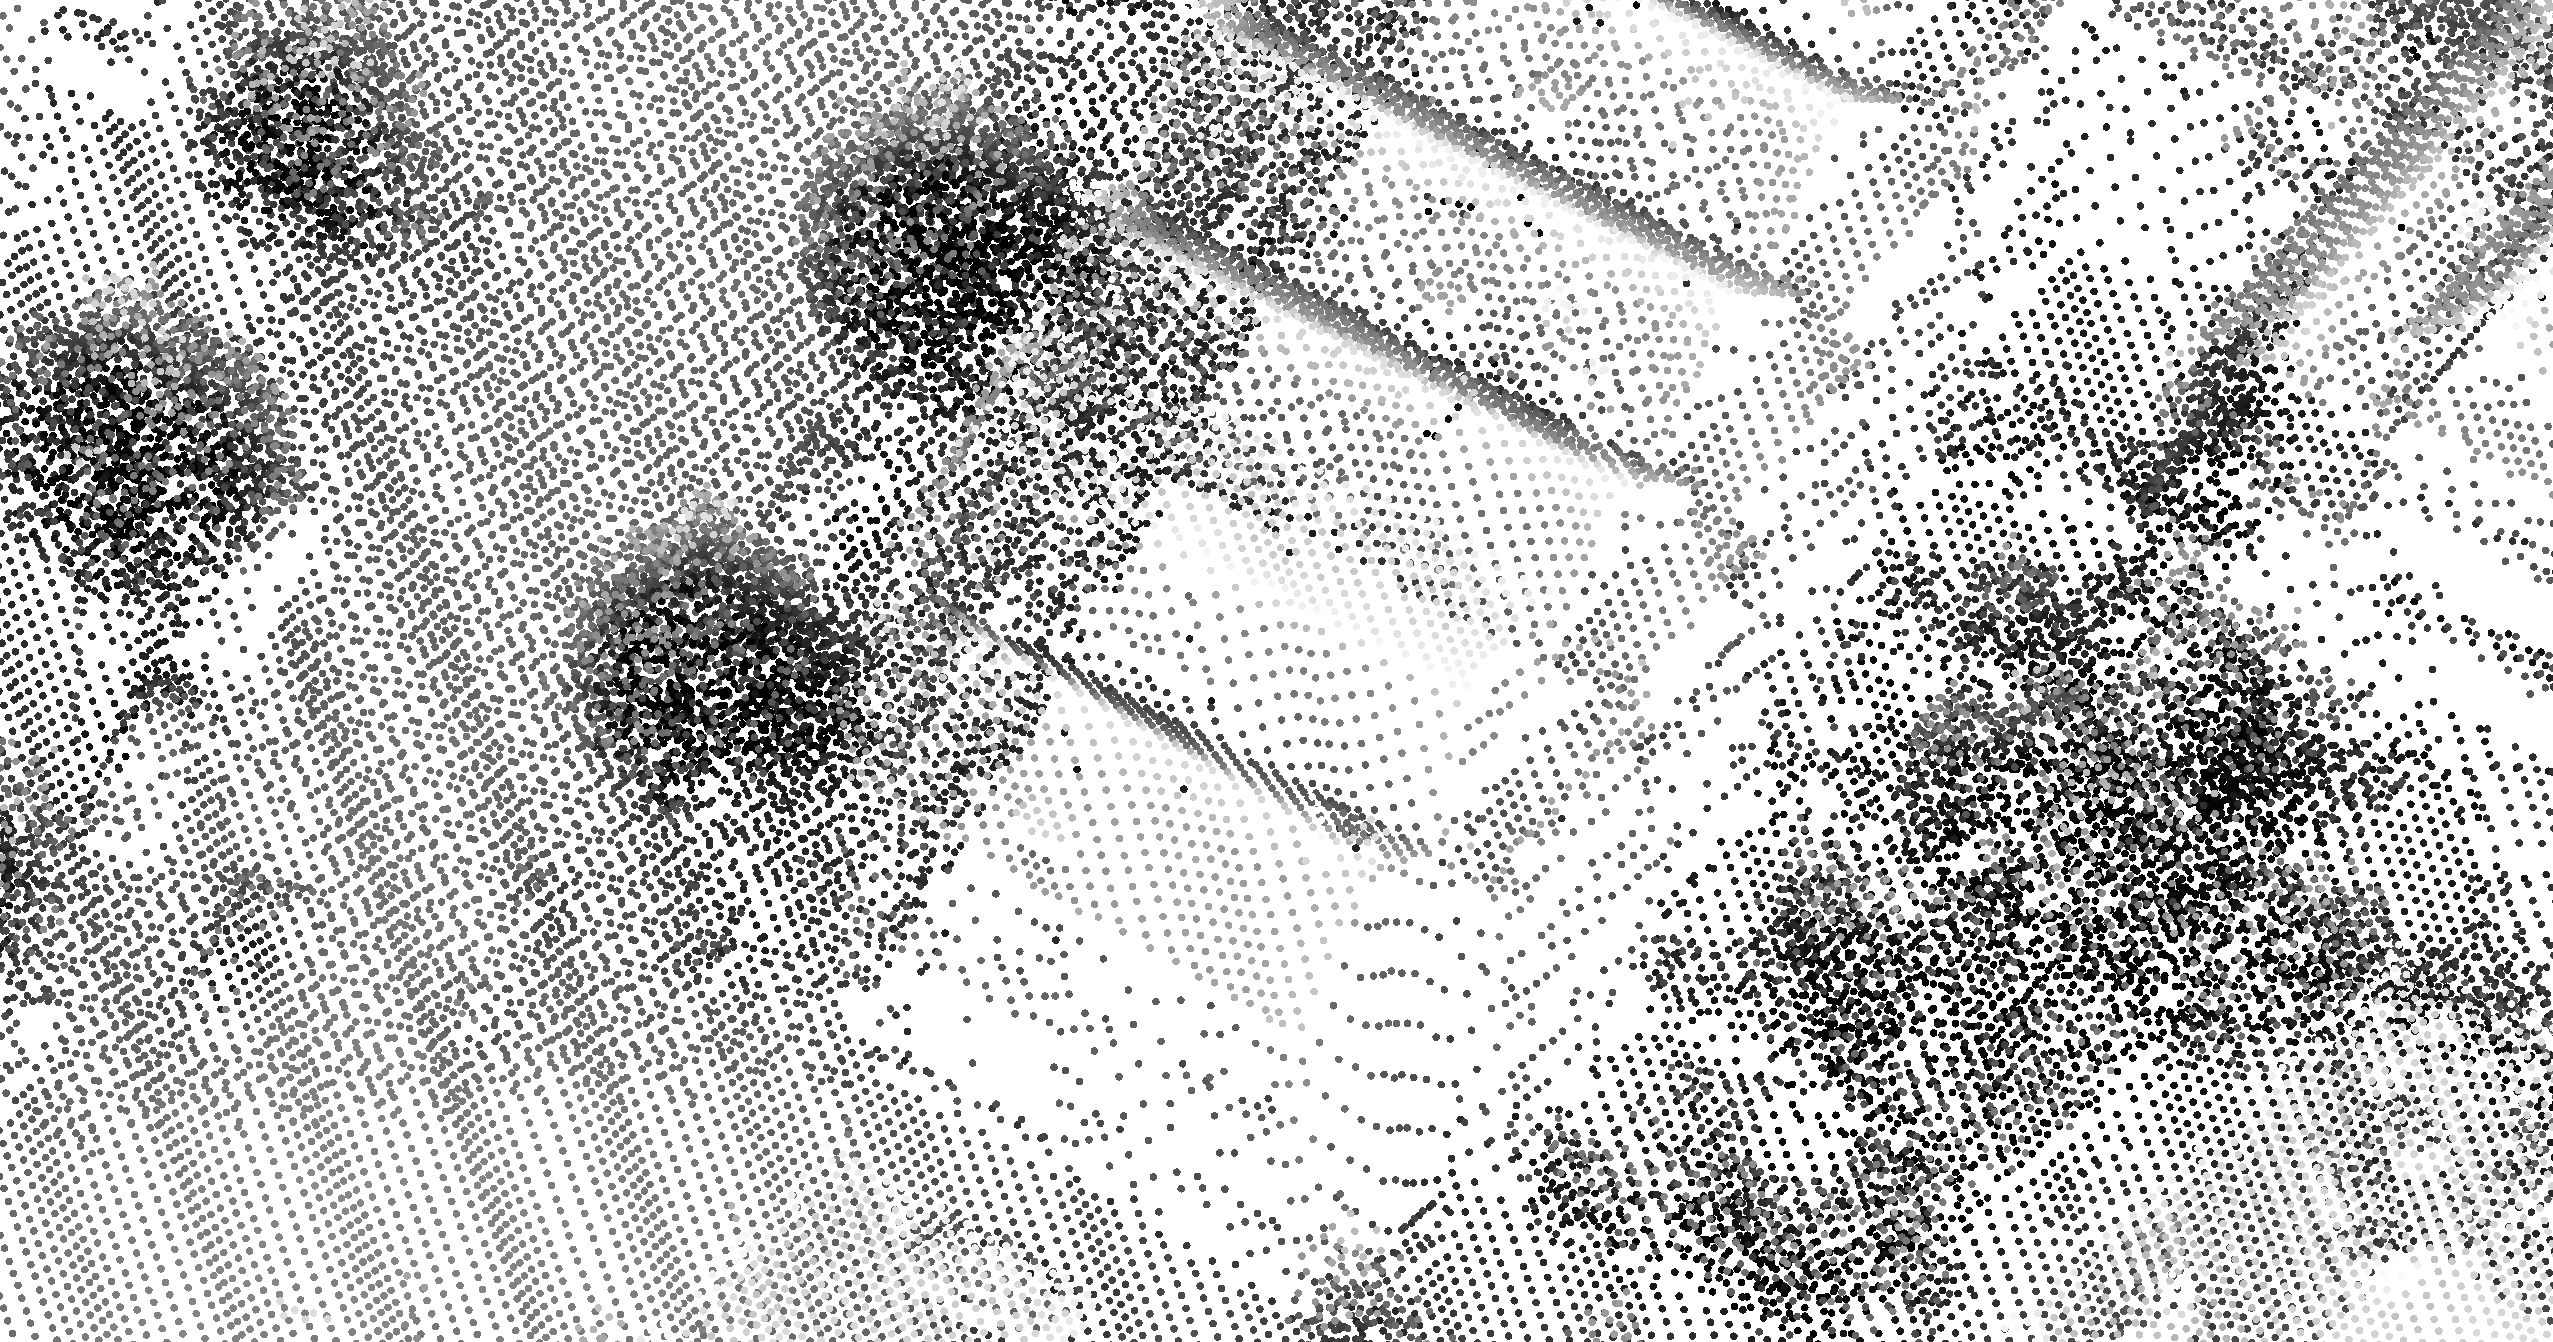
\includegraphics[width=\textwidth]{figs/ahn3_d.png}
		\subcaption{AHN3 (2014)}
		\label{fig:pcd:ahn3}
	\end{subfigure}
	\quad
	\begin{subfigure}{0.45\linewidth}
		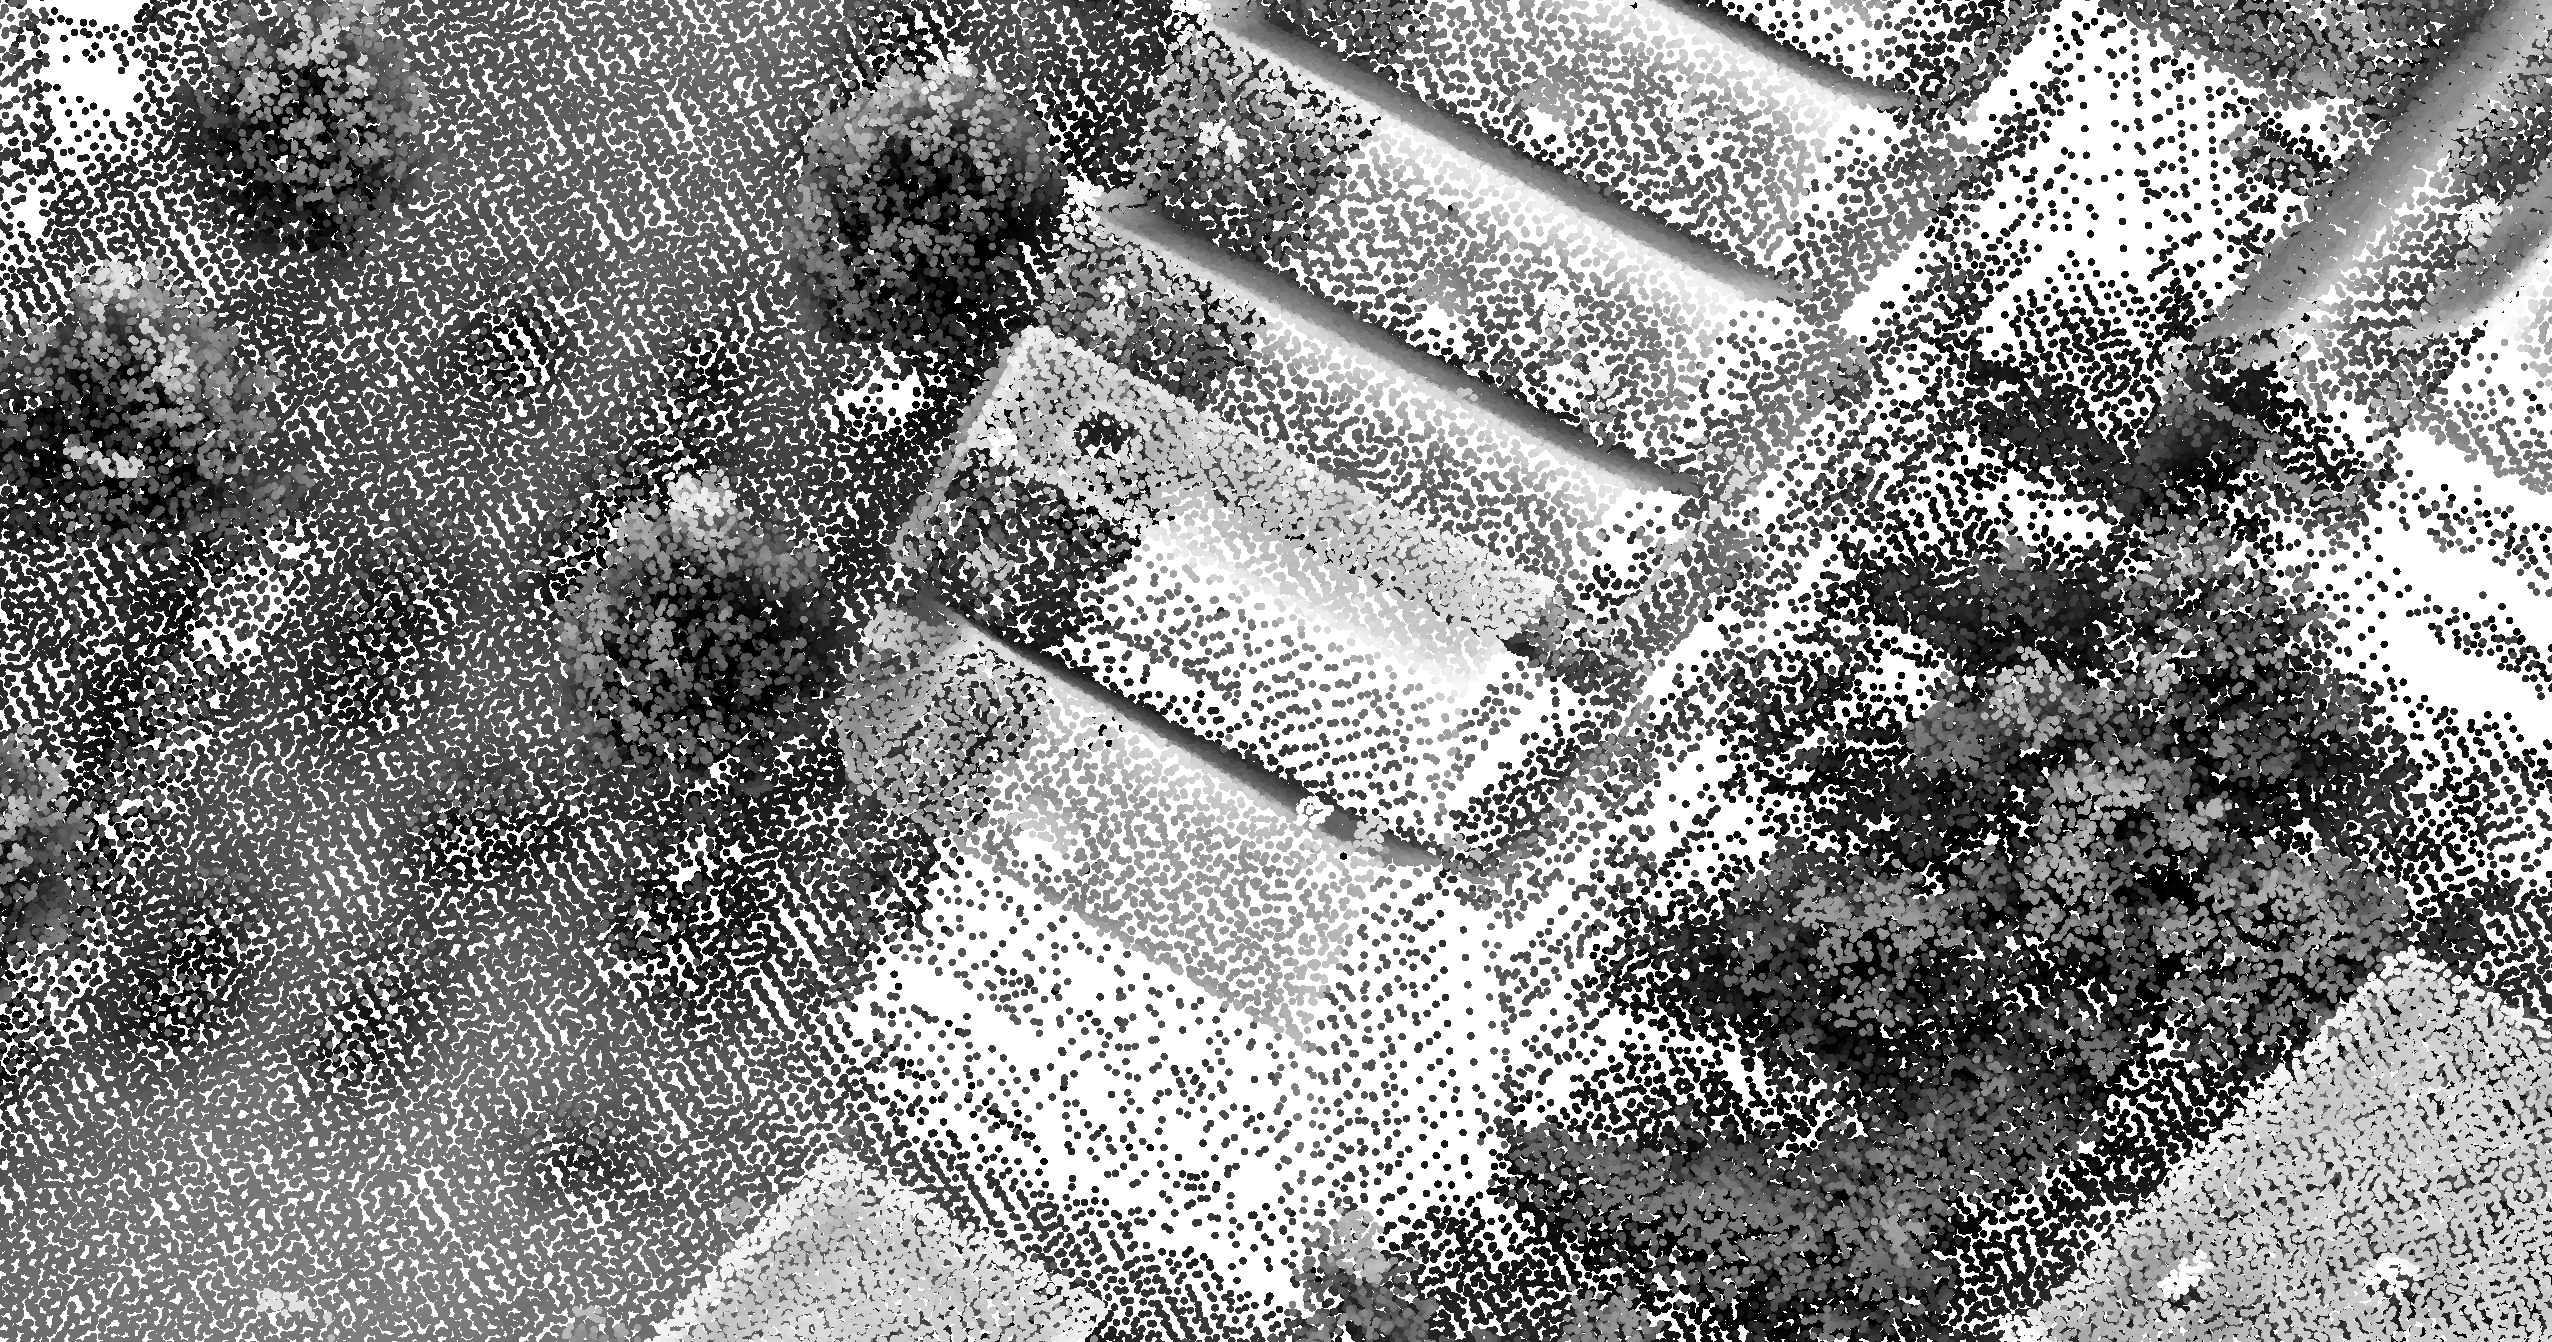
\includegraphics[width=\textwidth]{figs/rdam16_d.png}
		\subcaption{City of Rotterdam (2016)}
		\label{fig:pcd:rdam16}
	\end{subfigure}
	\caption{Several lidar point clouds for the same area in the city of Rotterdam. Point distribution and occlusion effects vary.}
  \label{fig:pcd}
\end{figure}

\subsubsection{Material properties}
Depending on material properties of a target surface, signals may be reflected in a way that makes it impossible to compute the correct distance. 
Surfaces that act like a mirror are especially problematic, Figure~\ref{fig:lidarAcquisitionConditions:b} illustrates this. 
First, it may happen that a pulse is reflected away from the sensor, \eg\ from a water surface, resulting in no distance measurement for that pulse. 
Or, in the case of photogrammetry, we will observe a different reflection in each image which heavily distorts the matching process, sometimes resulting in extreme outliers for water surfaces.  
In some cases, and only for active sensors, the reflected pulse does make its way back to the sensor, see for example the right half of Figure~\ref{fig:lidarAcquisitionConditions:b}. 
However, it will have travelled a longer distance than it should have and the scanner only knows in which direction it emitted the pulse. 
This effect is called \emph{multi-path} and the result is that points are measured at a distance that is too long and therefore they show up below the ground surface in the point cloud (see Figure~\ref{fig:outliers}).  
\begin{figure}
	\centering
	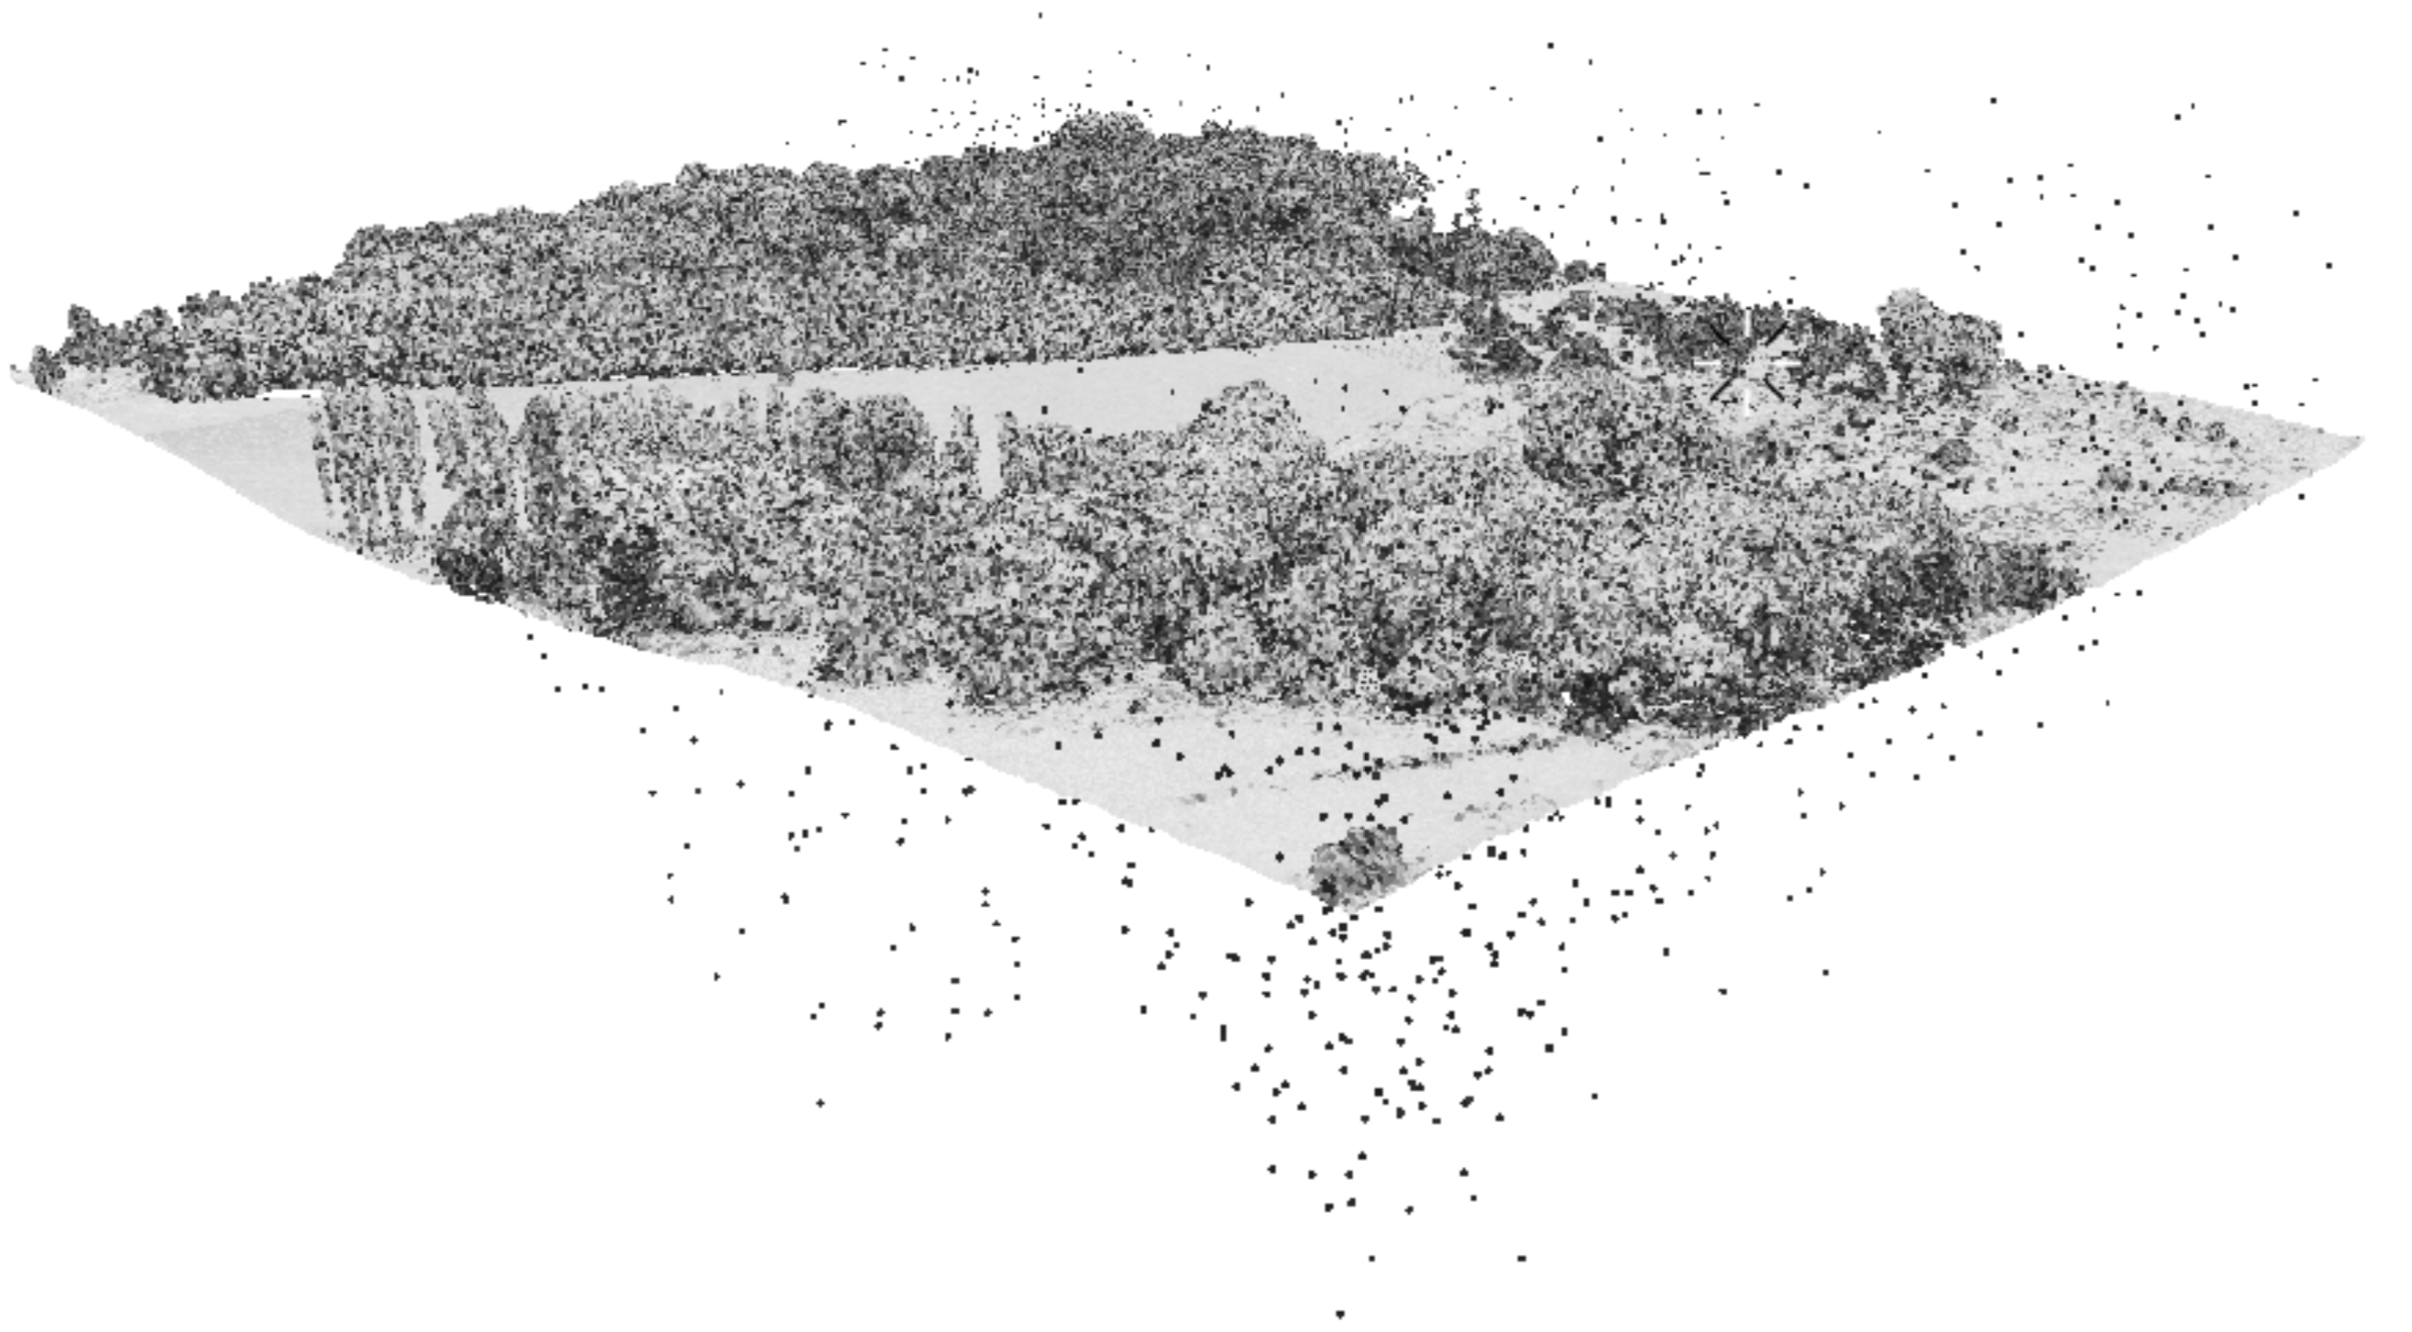
\includegraphics[width=\textwidth]{figs/outliers.png}
	\caption{Outliers, below and above the ground, in a lidar point cloud dataset.}
	\label{fig:outliers}
\end{figure}

Photogrammetry suffers from a few other problems as well, such as surfaces that have a homogeneous texture that make it impossible to find distinguishing features that can be used for matching. 
This may also happen in poor lightning conditions, for example in the shadow parts of an image.
%no texture (shadow), multi-path, complete absorption lightning conditions: shadow poor matching

\subsubsection{Moving objects}
An example of moving objects are flocks of birds flying in front of the scanner. These can cause outliers high above the ground, as illustrated in Figure~\ref{fig:outliers}.


\subsection{Processing}
It is common to perform some kind of process after acquisition in order to fix errors caused by the reasons mentioned above. 
In most cases such processes are largely successful. 
For instance, one can attempt to fill the void regions, sometimes referred to as \emph{no-data} regions, that are for instance due to pools of rainwater or occlusion, using an interpolation method (Figure~\ref{fig:voidfill}).
\begin{figure}
	\centering
	\begin{subfigure}{0.9\linewidth}
		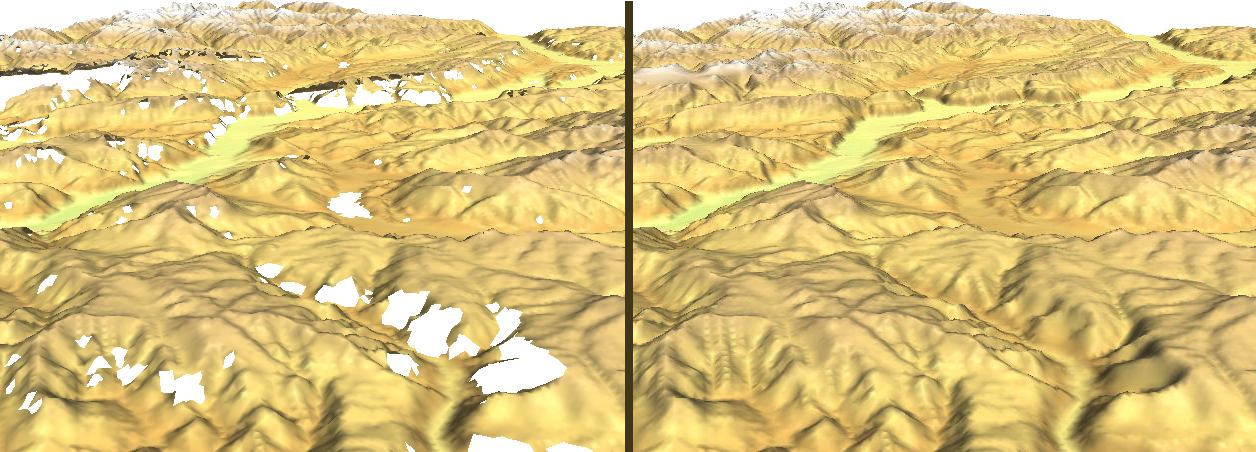
\includegraphics[width=\textwidth]{figs/srtm_trento_voidfill.png}
		\subcaption{Void-filling through interpolation in SRTM data}
		\label{fig:voidfill}
	\end{subfigure}
	
	\begin{subfigure}{0.9\linewidth}
		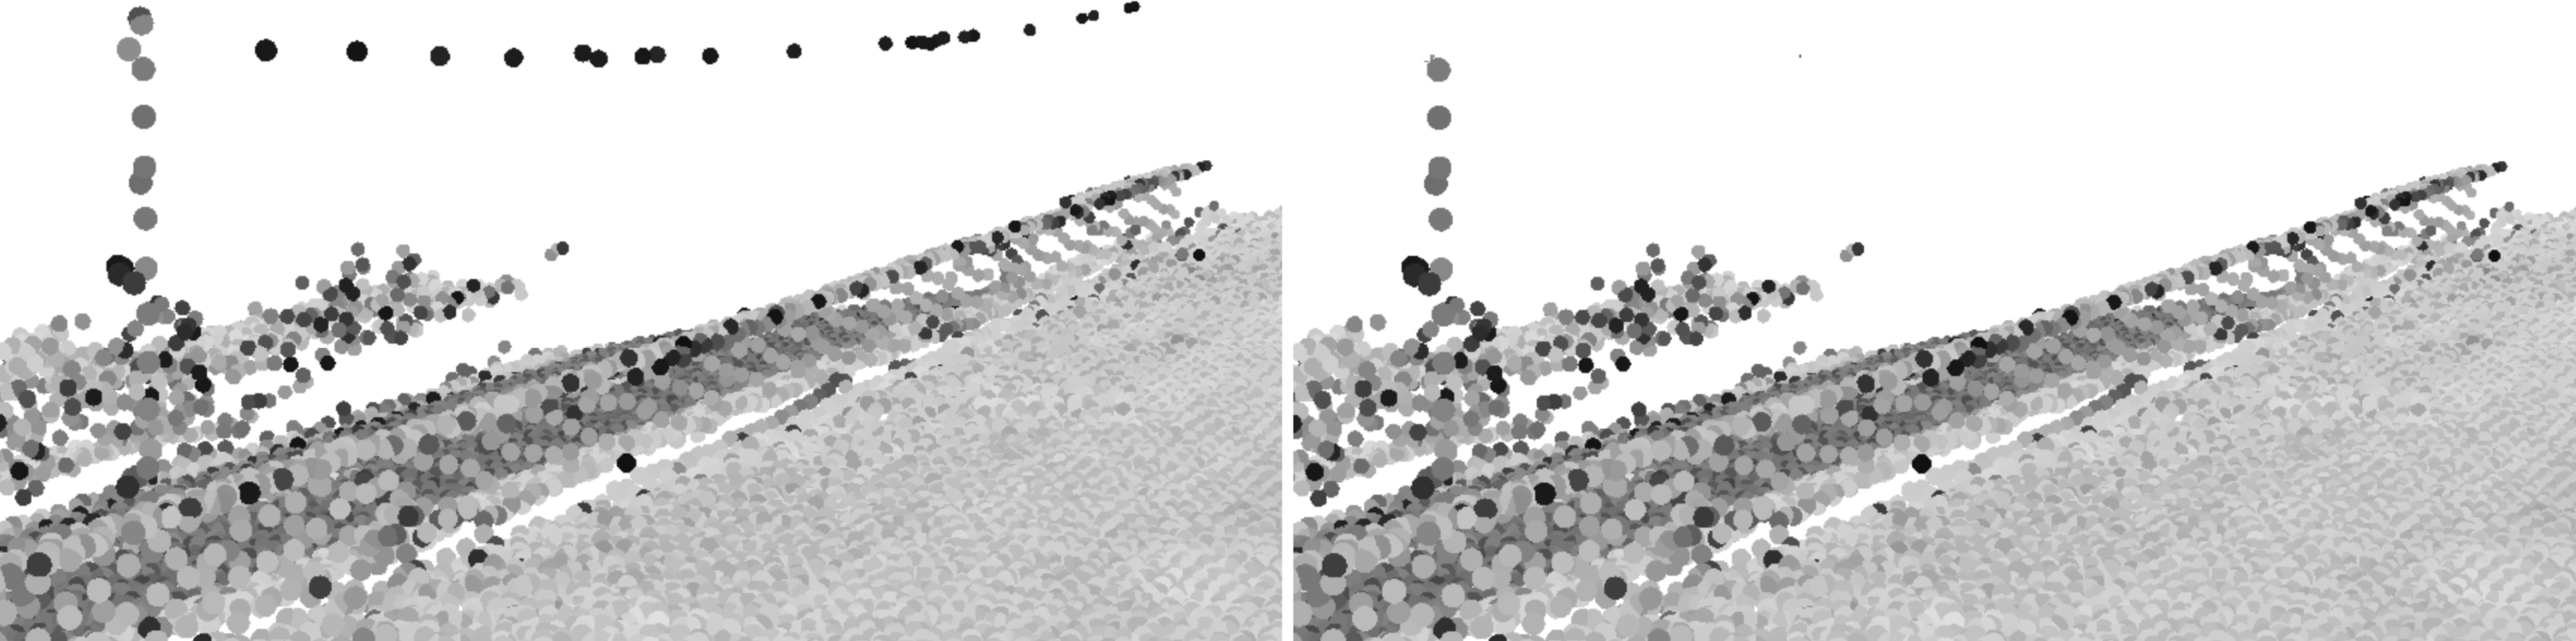
\includegraphics[width=\textwidth]{figs/ourlier-detection-wrong.png}
		\subcaption{Good points, \ie\ those on the power line, may be removed during outlier detection}
		\label{fig:outlier-wrong}
	\end{subfigure}
	\caption{Post-processing aimed at correcting artefacts. Before processing (left) and after processing (right).}
	\label{fig:processing}
\end{figure}
Or, one can attempt to detect and remove outliers caused \eg\  by multi-path effects or flocks of birds\footnote{This is a topic of lesson 12}. 
However, while the intention is always to reduce the number and severity of artefacts, these processes sometimes introduce distortions of their own.
For example, an outlier detection algorithm may remove `good' points if they look the same as outliers to the outlier detection algorithm (see \eg\ Figure~\ref{fig:outlier-wrong}).
And void-filling is only effective if the void area is not too large, since interpolation methods always assume there is sufficient neighbourhood information to work with\footnote{Chapters~\ref{chap:interpol} and~\ref{chap:kriging} explore the topic of spatial interpolation in detail.}.


\begin{link-box}
This is a paper that compares lidar and photogrammetry derived point clouds for the generation of a DEM\@. It shows that even when artefacts seem to be under control, both techniques may measure different elevations \citep{Ressl16}. 

PDF: \url{https://3d.bk.tudelft.nl/courses/geo1015/data/others/Ressl16.pdf}
\end{link-box}

%For instance, an outlier filter 
%misclassified points, smoothing effects in DIM

%Difficulties in automated DTM generation
%• Homogeneous areas and repeating structures;
% No distinct peak or multiple peaks of the similarity measures
%• Areas occluded in one image
% No correspondence exists;
%• Steep sloped surfaces
% Geometric difference between template and match window;
%• Discontinuities and break-lines
% No correspondence or geometric difference;
%• Non-lambertian surfaces
% Radiometric difference between template and match window;
%• Moving objects
% correct correspondence, incorrect elevation

% strip misalignment
% occlusion/geometry of target surface vs scanning position, density of points
% season- leaves on trees
% lightning conditions/shadow for photogrammetry
% surface material - reflactance, absorbance, multi echo, multiple returns


%few words about sensor fusion?


%%%
%
\section{Notes and comments}
If you would like to learn more about how a lidar scanner works, the article from \citet{Wehr99} is recommended.
More details on InSAR can be found in the manual from \citet{ESA07}.

\citet{Reuter09} give an elaborate overview of the processing that needs to be done to derive a high quality (raster) DTM from raw elevation measurements.

% fixing dem artefacts: https://www.sciencedirect.com/science/article/pii/S0166248108000044

%%%%%%%%%%%%%%%%%%%%
%
\section{Exercises}

\begin{enumerate}
	\item Name three differences between point cloud acquisition with lidar and with photogrammetry.
	\item Explain what the time-of-flight principle entails.
	\item How can you minimise occlusion effects in a point cloud during acquisition?
	\item Why does positioning, using e.g. GPS, play such an important role in acquisition?
\end{enumerate}